\scanpage{41}
\begin{tabular}{@{}l@{}}
\handwritten{Terminologie, notations\quad SGA 4\quad Vol. 2}\\
\handwritten{Attention, faire \uline{deux} listes disjointes !}
\end{tabular}
\figure{\begin{tikzpicture}
\draw (-5.8,.5)--(-5.8,-.7) .. controls (-2,-.95) and (3,-.8) .. (5.8,-.65)--(5.8,.7);
\end{tikzpicture}}

\begin{tabular}{@{}ll@{}}
(Sch)&VII 1.1\\
$\operatorname{Et}_{/X}\handwritten{,}\ X_{\mathrm{ét}}$&VII 1.2
\end{tabular}
\figure{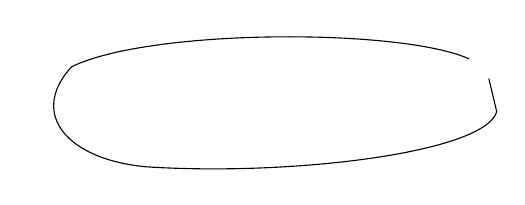
\begin{tikzpicture}
\draw (2.45,.55) .. controls (1.6,.94) and (-1.6,.94) .. (-2.6,.45) .. controls (-3.15,-.15) and (-2.65,-.73) .. (-1.65,-.82) .. controls (.2,-.94) and (2.65,-.64) .. (2.8,-.12)--(2.7,.3);
\end{tikzpicture}}

Topologie étale (sur (Sch), sur un schéma)\quad étale topology (on (Sch), \inserted{on a scheme)}\quad VII 1.2
\figure{\begin{tikzpicture}
\draw (1.8,.6) .. controls (.8,.47) and (-.3,.22) .. (-1.8,.05) .. controls (-2.1,.02) and (-2.12,-.25) .. (-1.98,-.47);
\draw (2.1,.08) .. controls (2.24,-.03) and (2.23,-.35) .. (2.05,-.55);
\end{tikzpicture}}

site étale d'un schéma\quad étale site of a scheme\quad VII 1.2

topos étale d'un schéma\quad étale topos of a scheme\quad VII 1.2

$f_{\mathrm{ét}}$\qquad VII \unsure{1\handwritten{,}\deleted{1}\handwritten{4}.4|1\handwritten{,}\deleted{L}\handwritten{4}4|1.\deleted{1.}4}
\figure{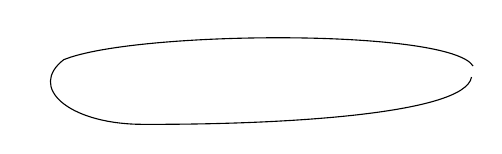
\begin{tikzpicture}
\draw (2.65,.22) .. controls (2.35,.7) and (-1.65,.67) .. (-2.55,.3) .. controls (-3,-.05) and (-2.5,-.5) .. (-1.6,-.52) .. controls (.15,-.53) and (2.55,-.4) .. (2.63,.08);
\end{tikzpicture}}

point géométrique d'un schéma\quad geometric point of a scheme\quad VIII 3.1.

foncteur fibre (relatif à un point géométrique d'un schéma)\quad fiber functor\deleted{\unsure{s}} (corresponding to a geometric point of a scheme)\quad VIII 3.3

$F_{\handwritten{\xi}}$\qquad VIII 3.3
\figure{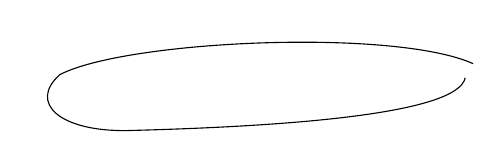
\begin{tikzpicture}
\draw (2.65,.2) .. controls (1.65,.65) and (-1.75,.5) .. (-2.6,.06) .. controls (-3,-.3) and (-2.6,-.66) .. (-1.75,-.65) .. controls (.2,-.6) and (2.45,-.45) .. (2.55,.02);
\end{tikzpicture}}

hensélien (anneau local - )\quad henselian local ring\quad VIII 4.1

\deleted{Clôture} henséli\unsure{\deleted{e}s|\deleted{s}e}\unsure{\deleted{n}é|\deleted{é}n}\deleted{\unsure{ne}} d'un anneau local\quad henselization of a local ring\quad VIII 4.1

strictement local (anneau)\quad strictly local ring\quad VIII 4.2

\figure{\begin{tikzpicture}[x=1cm,y=1cm]\draw (0,.02) .. controls (.1,.05) and (.13,.05) .. (.2,0);\draw (.3,0) -- (.75,.02);\draw (.85,.01) -- (1.05,-.02);\end{tikzpicture}} id \figure{\begin{tikzpicture}[x=1cm,y=1cm]\draw (1.8,.01) -- (1.9,-.02);\draw (2.05,-.03) .. controls (2.4,-.05) and (2.8,-.02) .. (2.9,.01);\end{tikzpicture}} (schéma)\quad strictly local scheme\quad VIII 4.2

anneau \unsure{\deleted{l}s|\deleted{s}l}trictement local (d'un schéma en un point géométrique)\quad strictly local ring (of a scheme \deleted{i}at a geometric point)\quad VIII 4.3

hensélisé strict d'un anneau local\quad strict hens\deleted{\unsure{\'{}}}elisation of a local ring\quad VIII 4.4

localisé strict d'un schéma en un point géométrique\quad strict localization of a scheme at a geometric point\quad VIII 4.3

flêche de spécialisation\quad speciali\deleted{s}zation \deleted{\unsure{morphism}}\inserted{arrow}\quad VIII 7.2

spécialisation d'un point géométrique\quad specialization of a geometric poin\unsure{t}\quad VIII 7.2
\figure{\begin{tikzpicture}
\draw[line width=.3pt] (.24,.58)--(.05,.07)--(-.1,-.46);
\end{tikzpicture}}

générisation d'un point géométrique\quad generization of a geometric point\quad VIII 7.2

$\overline{X}(\handwritten{\xi})$\quad ($\handwritten{\xi}$ point géométrique du schéma $X$)\quad VIII 7.1
\figure{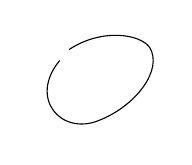
\begin{tikzpicture}
\draw (-.48,.31) .. controls (-.88,-.17) and (-.46,-.65) .. (.02,-.45) .. controls (.48,-.27) and (.84,.19) .. (.66,.48) .. controls (.53,.65) and (.05,.72) .. (-.36,.45);
\end{tikzpicture}}

Homomorphisme de spécialisation\quad \deleted{\unsure{a|f|t}} specialization homomorphism\quad VIII 7.7

\uline{Pt}$(E)$\qquad VIII 7.8.
\figure{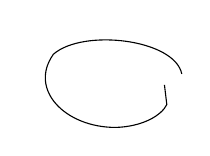
\begin{tikzpicture}
\draw (.87,.1) .. controls (.78,.54) and (-.38,.68) .. (-.76,.35) .. controls (-1.08,-.1) and (-.61,-.58) .. (.03,-.58) .. controls (.37,-.57) and (.61,-.43) .. (.68,-.29)--(.65,-.04);
\end{tikzpicture}}
% archive sheet number: 40
